%
% File coling2014.tex
%
% Contact: jwagner@computing.dcu.ie
%%
%% Based on the style files for ACL-2014, which were, in turn,
%% Based on the style files for ACL-2013, which were, in turn,
%% Based on the style files for ACL-2012, which were, in turn,
%% based on the style files for ACL-2011, which were, in turn, 
%% based on the style files for ACL-2010, which were, in turn, 
%% based on the style files for ACL-IJCNLP-2009, which were, in turn,
%% based on the style files for EACL-2009 and IJCNLP-2008...

%% Based on the style files for EACL 2006 by 
%%e.agirre@ehu.es or Sergi.Balari@uab.es
%% and that of ACL 08 by Joakim Nivre and Noah Smith

\documentclass[11pt]{article}
\usepackage{coling2014}
\usepackage{times}
\usepackage{url}
\usepackage{latexsym}
\usepackage{hyperref}
\usepackage{todonotes}
\usepackage{textcomp}
\usepackage{graphicx}
\graphicspath{ {images/} }
%\setlength\titlebox{5cm}

% You can expand the titlebox if you need extra space
% to show all the authors. Please do not make the titlebox
% smaller than 5cm (the original size); we will check this
% in the camera-ready version and ask you to change it back.

\newcommand{\changed}[1]{\textcolor{red}{#1}}
\newcommand{\TODO}[1]{\todo[inline]{{\footnotesize #1}}}

\title{An Overview over \\ Autonomous Vehicles}

\date{2016-04-22}

\begin{document}
\maketitle
\begin{abstract}
The introduction of Autonomous Vehicles promises a variety of profound advantages over conventional cars. Those advantages include increased safety, decreased individual transportation cost, mobility for everyone and possibly decreased energy consumption and emissions. 

The release of fully autonomous vehicles has been announced for the near future by a majority of car manufacturers. We give an overview over how current state of the art AVs, which are not yet commercially available, use sensors and machine learning learning approaches for autonomous driving.

We highlight open questions and active fields of research, important aspects of which are autonomous ethical decision making, liability issues and possible disruption of parts of the current job market.
\end{abstract}

\section{Introduction}
Soon, \textit{Autonomous Vehicles} (AVs) will traverse the streets of Gothenburg \todo{maybe add a reference / link here?}, and what has once been regarded as the transportation of the future is coming closer to being a part of today's reality. 

Among the earlier uses of the technologies used in the AVs of today was during the DARPA Grand Challenge \todo{confusing sentence}, where the challenge was to develop an AV capable of completing a 142-mile course of unrehearsed off-road terrain. The robot Stanley was the first to finish the race in 2005. Stanley used a combination of GPS and several sensors, such as RADAR mounted on the roof, to get an accurate position and used laser terrain mapping to identify obstacles on the path \cite{Thrun2006stanley}. This is an approach that is similar to how AVs work today, \changed{which we summarize in Section \ref{sec:howavswork}}. However, Stanley was designed for a static environment and would be unable to travel on populated roads, due to the difficulties and dangers accompanied with sharing space with pedestrians and other drivers.

Along with the technological difficulties \changed{the developers of AVs} face both ethical and legal questions, such as who is responsible in the event of an accident or where to crash in the case it's unavoidable. \changed{Machine ethics is one of the fields where a lot questions are still unanswered, and we discuss some of them in Section \ref{sec:ethics}}.

The dream of self-driving cars does however hold many promises, with one of it's bigger points being safety. In 2011 more than 2.2 million injuries were caused by automobile crashes in the United States alone \cite[p. 14]{Anderson2014rand}, while more than 39 percent of all fatalities involved alcohol \cite[p. 16]{Anderson2014rand}. With a far greater field of vision, reaction time and control of safety-critical functions, the hope is that AV could drastically reduce these statistics. 

In this essay we intend to answer the questions of how the technology works today, whether or not it will change our life in a positive way and what problems still needs to be addressed as well as how the current technology handles those problems.

\section{How AVs work}
\label{sec:howavswork}
In order to get autonomous vehicles onto the road, many different technologies need to be combined into one final product. We give a description of these technologies and how they are encapsulated in the system as a whole in the following two subsections, one of which focuses on the sensors and the other on the software used in the car. The physical body of the car and the engine tend to be similar to normal cars. The focus of this section is on the Google self driving car.

\subsection{Sensors}
\changed{In order for an AV to navigate the real world, its software needs to obtain data about itself and its surroundings}. For that purpose, it has several types of sensors incorporated into its body. The software processes the data provided by those sensors to create a virtual representation of the real world which can then be used to calculate which actions to perform to reach its destination. There are two main types of sensors: Exterioceptive and proprioceptive. The former deals with information from the AV's environment, while the latter deals with information internal to the system \cite{BeesonTexas09}. Some examples of the data that can be obtained within each class are:
\begin{itemize}
	\item Extereoceptive: Distances to objects, object types, objects' speed and heading.
	\item Proprioceptive: Motor speed, wheel load, heading, position, battery status.
\end{itemize}
For a more functional perspective, the sensors can be organized into categories defined by its use cases for AVs:
\\\\\textbf{Know where you are going}:
\begin{itemize}
\item \textbf{GPS}: It allows the AV to determine its position in absolute terms. In optimal conditions it has good accuracy and precision, but it cannot be constantly relied on due to intermittent coverage caused by tunnels, canyons, buildings, radio interference, etc. \cite{SchweberMouser}
\item \textbf{IMU} (Inertial Measurement Unit): A type of dead-reckoning\footnote{Dead-reckoning is the process of estimating one's current position by using a previously determined position, and advancing that position based upon known speeds over elapsed time and course.} system using a 3-axis accelerometer providing data on linear motion, and a 3-axis gyroscope providing data on rotational motion. This data is then used to calculate the motion and relative position of the vehicle regardless of any sort of signal obstruction. It has good accuracy for short periods of time but has cumulative error so over time it gets very inaccurate. \cite{SchweberMouser}\cite{HellstromUmea}
\item \textbf{Compass}: It can be used to determine the AV's heading. It has good accuracy which doesn't change over time but it is subject to interference by magnetic objects and electrical sources. It also can be slow to settle except for the most expensive types. \cite{HellstromUmea}\cite{BeesonTexas09}
\item \textbf{Ground speed RADAR}: Measures real ground speed using the Doppler effect. It can be used for dead-reckoning. \cite{HellstromUmea}
\item \textbf{Wheel odometry}: Used for dead-reckoning. Uses optical encoders to measure the speed of the wheels and the direction of the steering wheel from which the relative position of the AV can be calculated. \cite{HellstromUmea}\cite{BeesonTexas09}
\end{itemize}
$~$\\
\textbf{See where you are going}:
\begin{itemize}
\item \textbf{LIDAR}: The device emits laser pulses, and measures the time the beam takes to reflect back to the sensor (Time-of-flight), then it calculates the distance using that measurement. By using a rotating, scanning mirror assembly on top of the AV, it provides 3D 360{\textdegree} view suitable for ``big picture'' imaging. It is not very effective for close-in control\todo{what's that?}. \cite{SchweberMouser}\cite{BeesonTexas09}
\item \textbf{Cameras}: They are typically used to enhance the resolution of the 3D information obtained by the LIDAR, as well as detecting street signs and road markings. Their effectiveness is reduced by bad visibility conditions such as dusk, bad weather and dirt on the lens. \cite{SchweberMouser}\cite{HellstromUmea}
\item \textbf{RADAR}: Similar to LIDAR but instead of laser it uses a normal radio wave beam (usually 77GHz) to measure distance. It is used for close-in control instead of LIDAR: Parking, lane-changing and bumper-to-bumper traffic. \cite{SchweberMouser}\cite{BeesonTexas09}\cite{HellstromUmea}
\end{itemize}
$~$\\
\textbf{Get where you are going}:
Other sensors are needed for the correct operation of the AV, which deal with the internal state of the vehicle, such as: Battery \& fuel level sensors, engine temperature, oil pressure, etc.

Sensors are not perfect, they have reliability issues and the data provided is generally noisy. It is therefore common to use sensor fusion, a probabilistic approach to sensor reading in which each sensor readout gives a probability for the results, which are then fused into a combined result. The resulting information has lower uncertainty than what could be achieved by using these sources individually. \cite{HellstromUmea}

\subsection{Software}
In order to use the sensors to drive, humans need to program how to interpret all the data the sensors collect. With this information, the AVs need to focus on the two main accpects of operating the car, driving and avoiding all other objects. The cars use the information from the sensors to determine where they are, by combining it with information obtained from very specific maps that Google creates by collecting large amounts of data. These maps include everything about an area including curb height, intersection width, and lane layout \cite{chrisurmson2016}.
The cars determine where they are in real time by matching the images from the sensors to a specific place on the map and by incorporating where the car was a few seconds ago. While the cars rely on the maps immensely, they are programed to expect some change: when something in a cars surrounding is different than the preprogrammed map, they send the differences back to Google. Every detail from current construction sites to changes in the road due to erosion is reported \cite{chrisurmson2016}. The preinstalled maps are not a perfect solution. This is reflected in the fact that those AVs are not able to drive in snow, because the snow changes the landscape and therefore the physical markers Google uses for localisation \cite{chrisurmson2016}. 


After the cars locate exactly where they are, they need to worry about following road rules. Many of these driving rules are trivial and just need to be programmed
into the car. With the help of the very detailed maps that show things like stoplights, stop signs, and speed limits, the cars can deduce the correct and
law abiding action. However, to drive safely, the cars also need to be aware of everything else on the road, i.e. to identify and specify all other nonnative objects. Once they recognize that there is something in the surrounding area the computers use machine learning techniques to differentiate between every possibility \cite{zhu2012object}, where the three main categories for classification are cars, pedestrians and cyclists.
Within those categories there are more specific categorizations, for example the cars differentiate between, trucks or road workers in orange vests \cite{zhu2012object}. They also look out for common things in the road like traffic cones. As shown in Figure 1, the car recognizes many objects including cars and bikers. All the purple boxes are other cars, the light blue box in the bottom right of the intersection is thought to be a human. Once the car guesses what type of object something is, it starts to make assumptions about what the object will do next. These guesses are usually pretty simple: if a car is driving straight, it assumes the car will continue to drive straight and if a car is in the turning lane it will probably turn. The cars are programmed to anticipate the next move while also keeping in mind that other drivers might do something different \cite{chrisurmson2016}. The long green and red cuboids shown in Figure 1 are the projections of other vehicles that might interfere with the autonomous vehicle's current path. In case the car sees something in the road that is cannot recognize, it stops. Unlike a human, the car has no problem focusing on and predicting directions of many different cars at once. 
\begin{figure}[!ht]
  \centering
      \reflectbox{%
                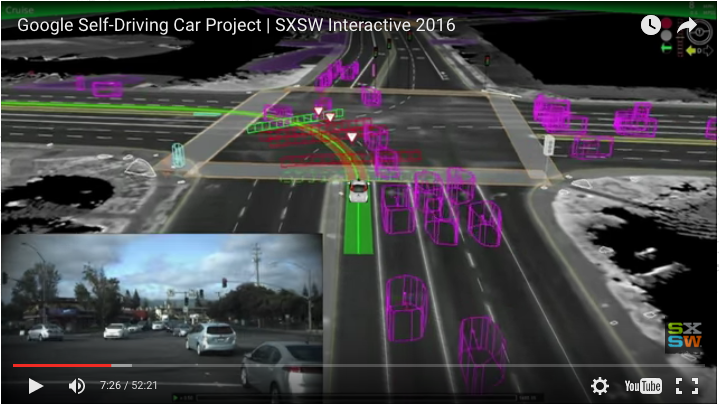
\includegraphics[width=0.7\textwidth]{drivingcar}}

\caption{The small box to the right is a picture from the front window of the car. The rest of the image is how the car interprets images from the sensors. The purple boxes are other motored vehicles. The blue box on the crosswalk is a person. The green track is where the car is planning on driving. The long green and red cuboids are the projected motion of cars that would end up in the  path of the car \cite{chrisurmson2016}}.
\end{figure}


Because AV cars are programmed to take specified actions under specific circumstances, it is relativity easy to predict how they will act. While they are far from perfect, Google has gone very far to make them at least as reliable as human drivers. This is reflected by the number of accidents the cars have caused so far: they have driven 2.4 million kilometres on public roads, whereat they have been considered at fault for exactly one car accident \cite{chrisurmson2016}. While more kilometres need to be driven before it can be argued that they are safer than human drivers, the numbers are pointing in that direction. 

\section{Social and Ethical Implications of AVs}
\paragraph{Impact on the society in general.}
The introduction of autonomous vehicles could drastically decrease the individual cost of transportation, especially because the passenger can use the transportation time for work or other activities. According to Anderson et al. this will most likely lead to ``low-density patterns of land-use surrounding metropolitan regions'' \cite{Anderson2014rand}, because longer distances to the workplace will be acceptable.

The overall effect on energy consumption and emissions is unclear: on the one hand, the total vehicle miles traveled might increase due to reduced opportunity cost for time spent in the car. On the other hand, the technology also offers various possibilities to decrease emissions, including light-weight vehicles and \changed{platooning, where the distance between consecutive vehicles is reduced drastically}.

AVs could bring independence and mitigated social isolation for those unwilling or unable to drive. Note however that for this to actually make a difference, society has to ensure that all members of society can actually profit from the new technology.

\paragraph{Economics.}
Many jobs and a variety of professions will likely be affected by the introduction of AVs. In 2015, roughly 1.18 million bus and truck drivers have been employed in the US according to the Bureau of Labor Statistics \cite{USLabourBureau2016}, and those are only two examples of professions which would obviously be affected in a very direct way. Decreasing crash risks could impair the business of many insurance companies, and since AVs could facilitate the introduction of alternative fuels, jobs related to combustion engines might become obsolete. According to Anderson et al. ``... lost jobs might be replaced by others, perhaps related to the AV industry, but there may be considerable economic disruption'' \cite[p. 40ff]{Anderson2014rand}. Not only technical solutions are necessary here, but also appropriate policy reactions and extensive discussion and changes in society. The impact of automization on the labour market and possible policy reactions, including a basic income, are currently being discussed controversially \cite{VanDerVeen2002, Olsen2014}.

AVs will, just like most state-of-the-art technology, likely be very expensive in the first years. Thus, this presumably safe, fast, reliable and convenient mean of transportation might be only available to the richer parts of the population. Driving conventional cars could become a necessity for the poor, further increasing the social gap between rich and poor \cite[p. 39]{Anderson2014rand}.

\paragraph{Liability.}
The AV manufacturer's liability will likely increase, which, according to Anderson et al. ``could lead to inefficient delays in adoption of this technology''. Amongst others companies, Volvo has stated that it accepts full liability for accidents caused by their AV technology \cite{HarrisVolvo2015}. Manufacturers could try to mitigate the risks involved in accident liability by providing vehicles as a service instead of as a product. In any case, states will have to establish legal frameworks for autonomous driving. There is a wide range of possible policy toolkits, ranging from a federal insurance backstop in order to avoid delays in technology adoption, to simply assigning liability to human drivers.

\paragraph{Ethical Decision Making.}
\label{sec:ethics}
In a study on ethical decision making during AV crashes, Goodall comes to the conclusion that $(1)$ AVs would almost certainly crash, $(2)$ that an AV's decisions that preceded certain crashes have a moral component, and that $(3)$ there is no obvious way to encode complex human morals effectively in software \cite{Goodall2014ethical}. \changed{Goodall divides current approaches to machine ethics into two groups: rational and \textit{Artificial Intelligence} (AI) approaches.}

In the former, an AV must either adhere to a predefined set of rules or try to minimize some clearly defined function, which usually represents the total damage to humans, environment and property. These approaches are easy to implement and tailor-made for execution by computers, but the incompleteness of any set of rules and the difficulty involved in the articulation of complex human ethics as a set of rules are problematic. No matter how many rules are fed into such a system, there will always be situations in which the resulting behaviour does not match the expectations of human ethics.

The basic idea of AI approaches to AV ethics is to train a \textit{neural network} (NN) on a combination of simulations and recordings of real crashes, with human feedback on the ethical response. This \changed{eliminates} the problem of having to encode the complex human ethics into a mathematical set of rules. However, the inconsistency between how humans actually behave and what they believe, and lacking traceability (why did the NN decide the way it did in an accident?) involve a risk of missing transparency and manipulation. NNs capable of providing natural-language feedback of how they came to certain decisions are a active field of research \cite[p. 63]{Goodall2014ethical}.

Goodall proposes a three-phase ethical vehicle deployment strategy \cite[p.63]{Goodall2014ethical} which can be compared to the moral education of a child. \changed{Those phases are not supposed to be interpreted as a timed technological roadmap, but rather as rough guidance for society in general, and the AV development community in particular. The phases are to be implemented as the corresponding technology becomes available}. In the first phase, rational ethics are used, i.e. the AV must follow some clearly defined set of rules. In the second phase, a hybrid rational and AI approach is used: The strict rules from phase one remain active as a boundary, but additionally the complex specifics of human ethics are learned using AI technology. In the third phase, once the technical obstacles have been overcome, natural language feedback should be added to the AI technology of phase two. \changed{The presented approach can be compared to the behaviour of parents who usually try to give their children the possibility to think about and develop their own morals, while still enforcing some boundaries.} Current state-of-the-art AVs are in the first of these three phases, whereat active research is happening in all of them.

\changed{The approach presented by Goodall by itself does not solve any of the aforementioned problems regarding the ethical decision making of AVs. Instead, it offers a framework that is supposed to allow for continuous development in this to a very large extent open field of research. }

\section{Conclusion}
In conclusion, AVs need a operational, ethical, and legal structure to become commonplace on roads. The technology for AVs has gotten incredibly far in the past decade. As of 2016, cars can drive successfully and safely using exteroceptive and proprioceptive sensors in combination with programmed driving rules and machine learning techniques. Even though corporations like Volvo have acknowledged that their liability will increase as a direct result of producing AVs, they are still enthusiastically embracing this technology. Once the technology has reached the third phase described by Goodall\todo{refering to this here is a bad idea, since a reader should be able to read abstract + conclusion only}, AVs should be able to make their own ethical decisions. Overall most of these condition are close to being met. 

When these conditions are met AVs will be not only a technological milestone but also a social and cultural breakthrough. It could cause a demographic distribution change as well as an increase in time available for commuters to work or other things. Moreover it will cause an overhaul of the transportation sector. Lastly it will change the lifes of people incapable of driving. AVs could impact lives immensely. 

Given time, we believe that AVs will face all their problems and prove themselves. Although there are still a few issues, the implications of AVs could have an incredibly positive impact on society. 


% BibTeX 
\bibliographystyle{IEEEtran}
%\bibliographystyle{acl}
\bibliography{Bibliography}


\end{document}

%%% Local Variables:
%%% mode: latex
%%% TeX-master: t
%%% End:
